\section{Code Structure}
\subsection{Designed Work Flow}
There are three main sections to a CFD analysis; Meshing, Simulation, and Analysis. DSMC-PIC is a subsection of CFD, therefore the original developers have designed systems for all three sections. However, most  CFD analysis does not require the user to do all three tasks each time. There are many different analysis tasks on the same results from a simulation with a single mesh. There are many different simulations possible with the same mesh. Therefore, SINATRA was broken down into 3 parts according to the three tasks it is able to accomplish. Each of those sections have their own repository, source code, and executables. They also share a resources repository between them. This allows the user to work in the meshing system and create the mesh or meshes necessary for their task. Then they move to the simulation system and use the newly created meshes as part of the simulation input. Once they have simulated the domain, they can take the created output files and run different analysis codes or create their own for their specific task. 


% TO DO make sure that  cart3d has a 3d octree mesher
% TO DO - do I need trademark things here?

\begin{figure}
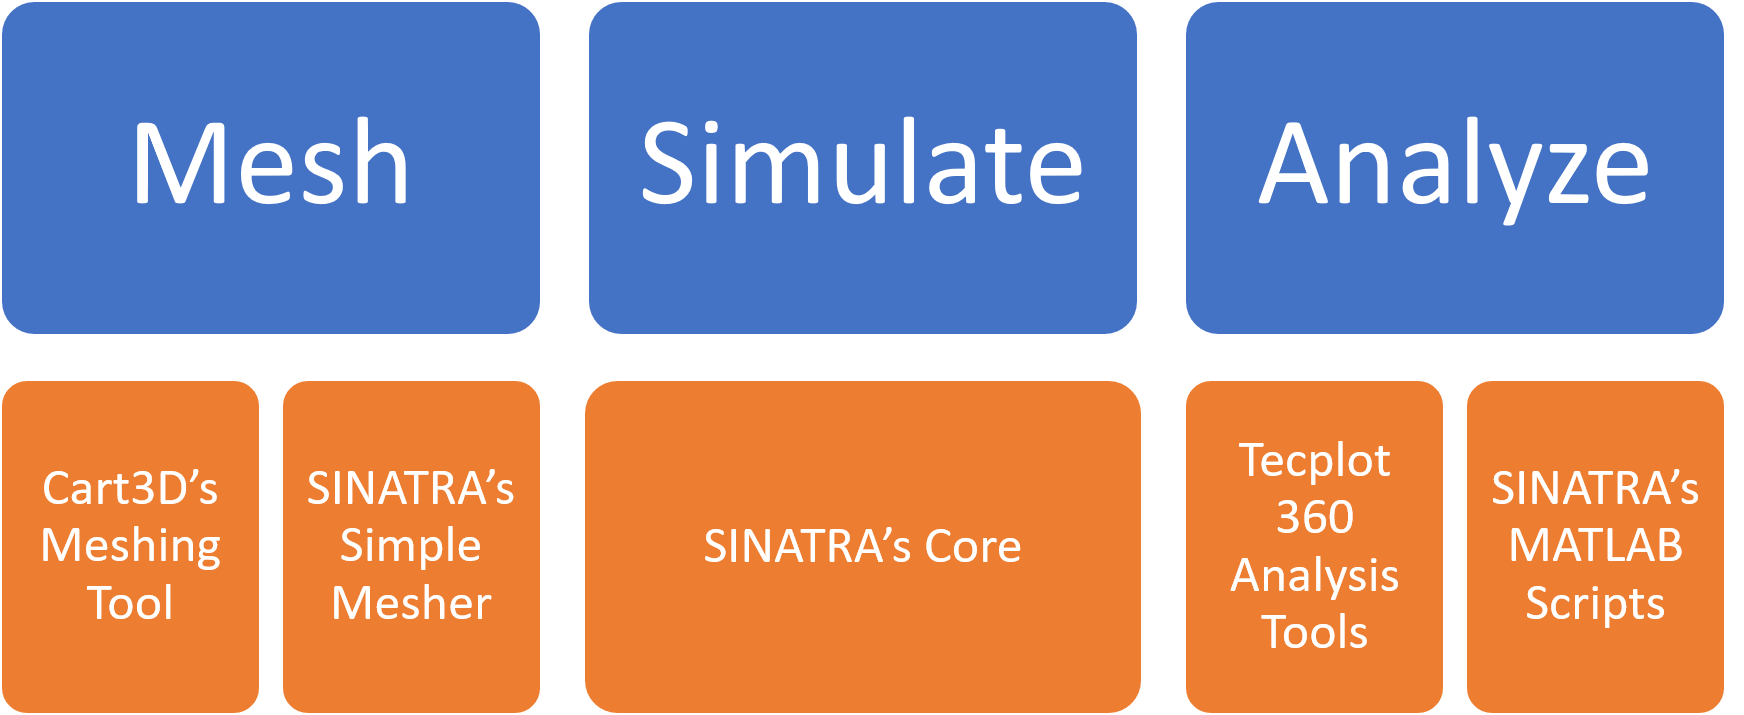
\includegraphics[width=.95\textwidth]{figures/UserWorkFlow.png}
\centering
\caption{Work flow System for SINATRA}
\label{fig:UserWorkFlow}
\end{figure}

\subsection{Mesh}
% TO DO talk about auto meshing and auto timesteps
% TO DO talk about new meshing with objects
The original developers have designed this work flow for SINATRA while including the option for third party software to be used for the meshing and analysis sections. As seen in figure \ref{fig:UserWorkFlow}, Cart3D\textsuperscript{TM} \cite{cart3d} was chosen to be the meshing 3rd party additional tool. Meshing a domain for SINATRA requires an Octree Mesh. For cases where the domain is empty, the homegrown SINATRA meshing tool is quick and simple. However, when an object is added to the domain, meshing becomes a much more complicated task; this is outside the scope and purpose of SINATRA. Cart3D\textsuperscript{TM} is a CFD analysis tool by NASA which is available to universities. It has within it a three-dimensional octree meshing tool which can take geometries and domain sizing as inputs. SINATRA will take the outputted mesh and use it for Simulations. Cart3D has not been tested with SINATRA. It has been slated for future work for another developer to fully integrate Cart3D\textsuperscript{TM} and geometry boundaries with SINATRA\footnote{It may be necessary to run Cart3D within a Linux\textsuperscript{TM} virtual box for Windows\textsuperscript{TM} users}. \par

\subsection{Simulation}

SINATRA has been designed to be simple to develop and execute. Execution is completed through one executable file and one input text file. For simplicity, Windows\textsuperscript{TM} users can drag the .txt file onto the .exe file to run the simulation. SINATRA was deliberately built to be machine independent to reduce the risk of the code not being developer further or used for new tasks. Therefore, the executable and output do not depend on using a specific Integrated Developer Environment like Visual Studio\textsuperscript{TM} or even using a certain operating system. A user can run many simulations or string together meshing, simulating, and analysis simply through a batch script. An example script is shown in Appendix \ref{app:examplescript}. \par
Because SINATRA was built to be platform independent, it is very easy to compile. It requires only a single command with zero libraries.\footnote{Need openmp for parallelization} There are sample compile statements in the ReadME and compile scripts, but even an intermediate C++ coder could figure out how to compile SINATRA from the file list alone. This helps new developers move quickly through the code learning phase and can even allow beginners to explore the code base and test more complicated features. SINATRA has been tested through being compiled with various compilers and on different operating systems.  

% TO DO add ppt graphic of this codeflow one with all the files and titles - appendix
% Future - add example of scripting all of them together

% TO DO talk about debugging and gdb

\subsection{Analysis}
% Future make simple tecplot analysis script
% TO dO add citattions of david and macs thesies
% TO DO make analysis functions which gooes through all the cells (send anamynous function)


 After the simulation phase is completed, the user can use the SINATRA output files for analysis. The original developers created MATLAB scripts within SINATRA which do basic types of analysis. For other analysis, Tecplot 360\textsuperscript{TM} \cite{tecplot} has been chosen as a third party tool. Tecplot\textsuperscript{TM} is a specific CFD analysis and visualization tool which can show the mesh, geometry, and fluid flow. It includes robust visualization and animation tools as well as various analysis functions. SINATRA can output data in a format which Tecplot\textsuperscript{TM} reads natively. Tecplot\textsuperscript{TM} and SINATRA's integration has been tested and used by the first developers.\par
 \indent SINATRA's analysis section has not been built with an encompassing set of features to complete any task. It is up to the future users to determine the analysis they need to accomplish, edit SINATRA's output class to accommodate, and compile the output data into the format they need. This can be completed through looking at SINATRA's output class and reformatting other analysis techniques for the task at hand. Tecplot\textsuperscript{TM} and the included MATLAB scripts can do a majority of the the beginning analysis, but the most detailed tools will need to be built by new developers. 


\subsection{Code Flow} % I think this goes somewhere else. another section. maybe beginning of electric
 
 
\subsection{Execution Time} % I think this goes under improvements...
A DSMC code is by nature a very computationally intense program. It requires a large amount of memory to store all of the data of each particle and mesh cell. It requires a lot of computational power to calculate the movement and collisions. Therefore, it is important to design the code to be efficient and powerful. This is why C++ and classes were chosen for SINATRA. However, it is still a slow simulation for a large meshes with high particle densities. It is slated as future work for a developer who specializes in computer science and computational optimization to reduce the execution time of large SINATRA runs. However, there are a few bottlenecks and available improvements which were added by the author. These help manage simulation time, especially when the Poisson equation solver is included.\par
The simplest and most effective way to reduce simulation time on a DSMC simulation is parallelization. Parallelization is a complex and involved field with many competing ideas on best practices. There are many discussions about best ways to parallelize DSMC codes and PIC codes. Parallelization itself is also on the forefront of new technology in this age. Moore's law has allowed programmers to have a large amount of memory for their simulation, so that is rarely the constricting factor. Processors seem to have become as powerful as they will be for user made systems on languages like C++\textsuperscript{TM}. However, breaking the simulation between multiple cores or even within the GPU seems to be the new normal for decreasing execution times. For SINATRA, there are many parallelization possibilities. It is slated for future work for another developer to optimize the parallelization capacity. At this time, simple parallelization has been developed by the author. During the particle propagation phase, there is no interaction between the commands. Therefore, it can be parallelized by using the library openmp\textsuperscript{TM} \cite{openmp}. This can be enabled through an optional keyword in the input file and ensuring the library is included in the compile statement. \par
Another simple process to reduce the execution time is during the linking phase. After the particles are created, they must be associated with the cells that they are in. To do this it requires a double for loop with particles inside cells. This is a very slow process. A few time reduction techniques have been implemented by the author. However, there is a simpler solution. There is an option in SINATRA to seed particles in a uniformly random way \cite{Galvez2018a}. This method creates the same number of particles in each cell but randomly distributes them within the cell. Therefore, this linking process can be removed completely and the execution time reduces significantly. \par
Finally, an important tool for execution time analysis is a profilier. A profilier allows the user to view exactly how often each line of code is run, how long it takes to run, and the subprocesses which contribute to that execution time. This is a strong way to identify simple coding bottlenecks and optimizing the coding time. The author has set up the compiling and code base in order to fit with the profilier Very Sleepy\textsuperscript{TM} \cite{Sleepy}. This is a light and simple profilier which shows each line of the source code and the timing involved. \par


% ADD table of a simulation with each of these items enabled
% Cite processer information
% Cite DSMC paralization papers

